\documentclass{article}
\usepackage[utf8]{inputenc}
\usepackage{graphicx}
\title{Cara Pembuatan Aplikasi di Oracle APEX}
\author{Almi Bachri (1184043) }
\date{Oktober 2019}

\begin{document}

\maketitle
\begin{enumerate}
    \item Login ke oracle APEX
    \begin{figure}[!htbp]
        \centering
        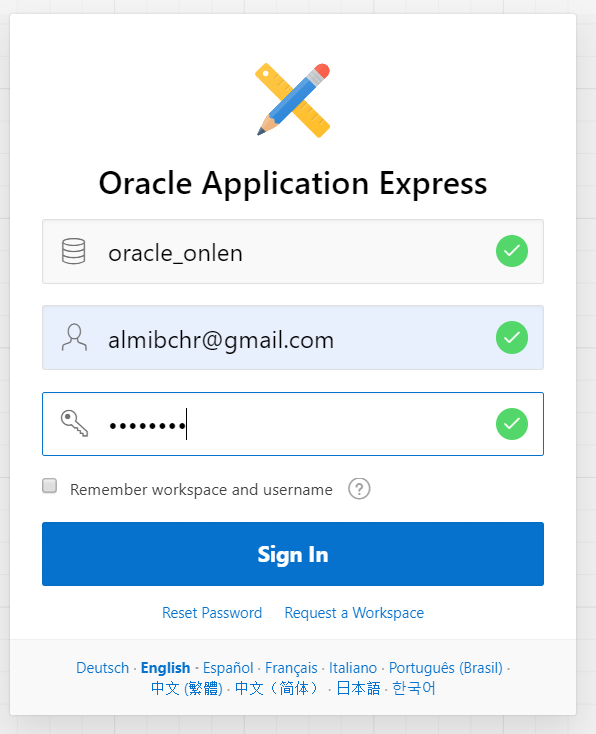
\includegraphics [width=6cm]{figure/Capture.PNG}
        \caption{Caption}
        \label{fig:my_label}
    \end{figure}
    
    \item Pilih "App Builder" lalu klik "Create"
     \begin{figure}[!htbp]
        \centering
        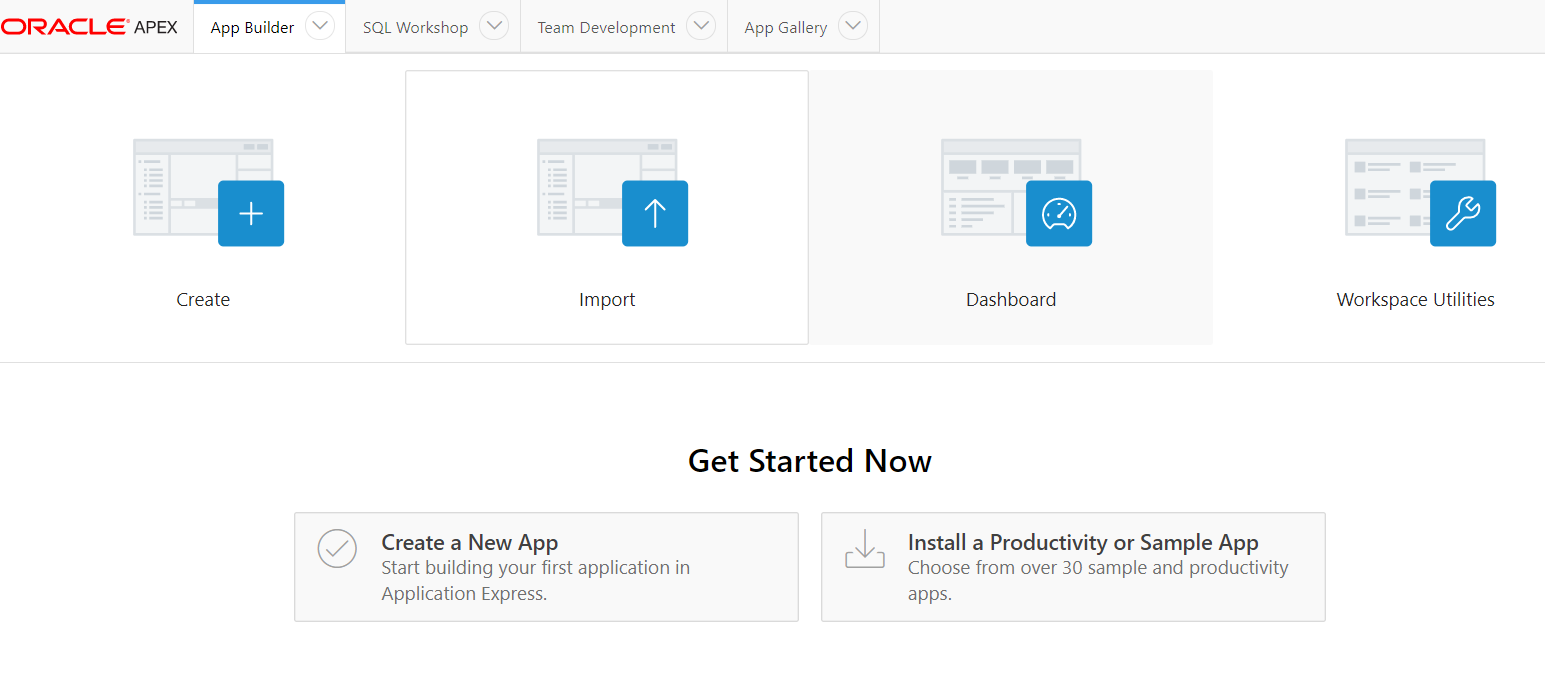
\includegraphics [width=7cm]{figure/Capture1.PNG}
        \caption{Caption}
        \label{fig:my_label}
    \end{figure}
    
    \item Klik "From a File"
     \begin{figure}[!htbp]
        \centering
        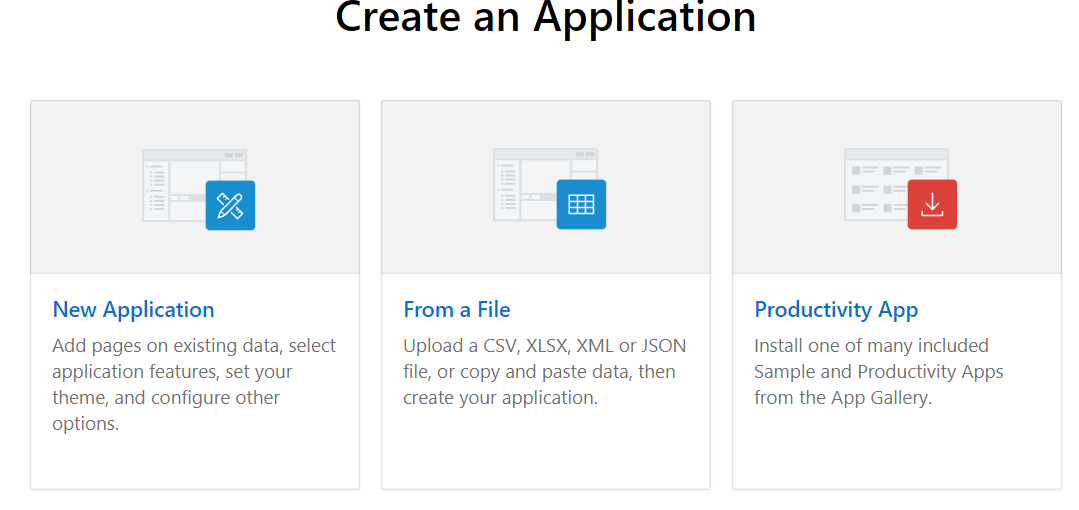
\includegraphics [width=8cm]{figure/Capture2.PNG}
        \caption{Caption}
        \label{fig:my_label}
    \end{figure}
    
    \item Masukkan file yang akan kalian buat, bisa "upload file" atau "copy and paste", kalau saya disini dengan cara "upload" file yang akan dibuat.
     \begin{figure}[!htbp]
        \centering
        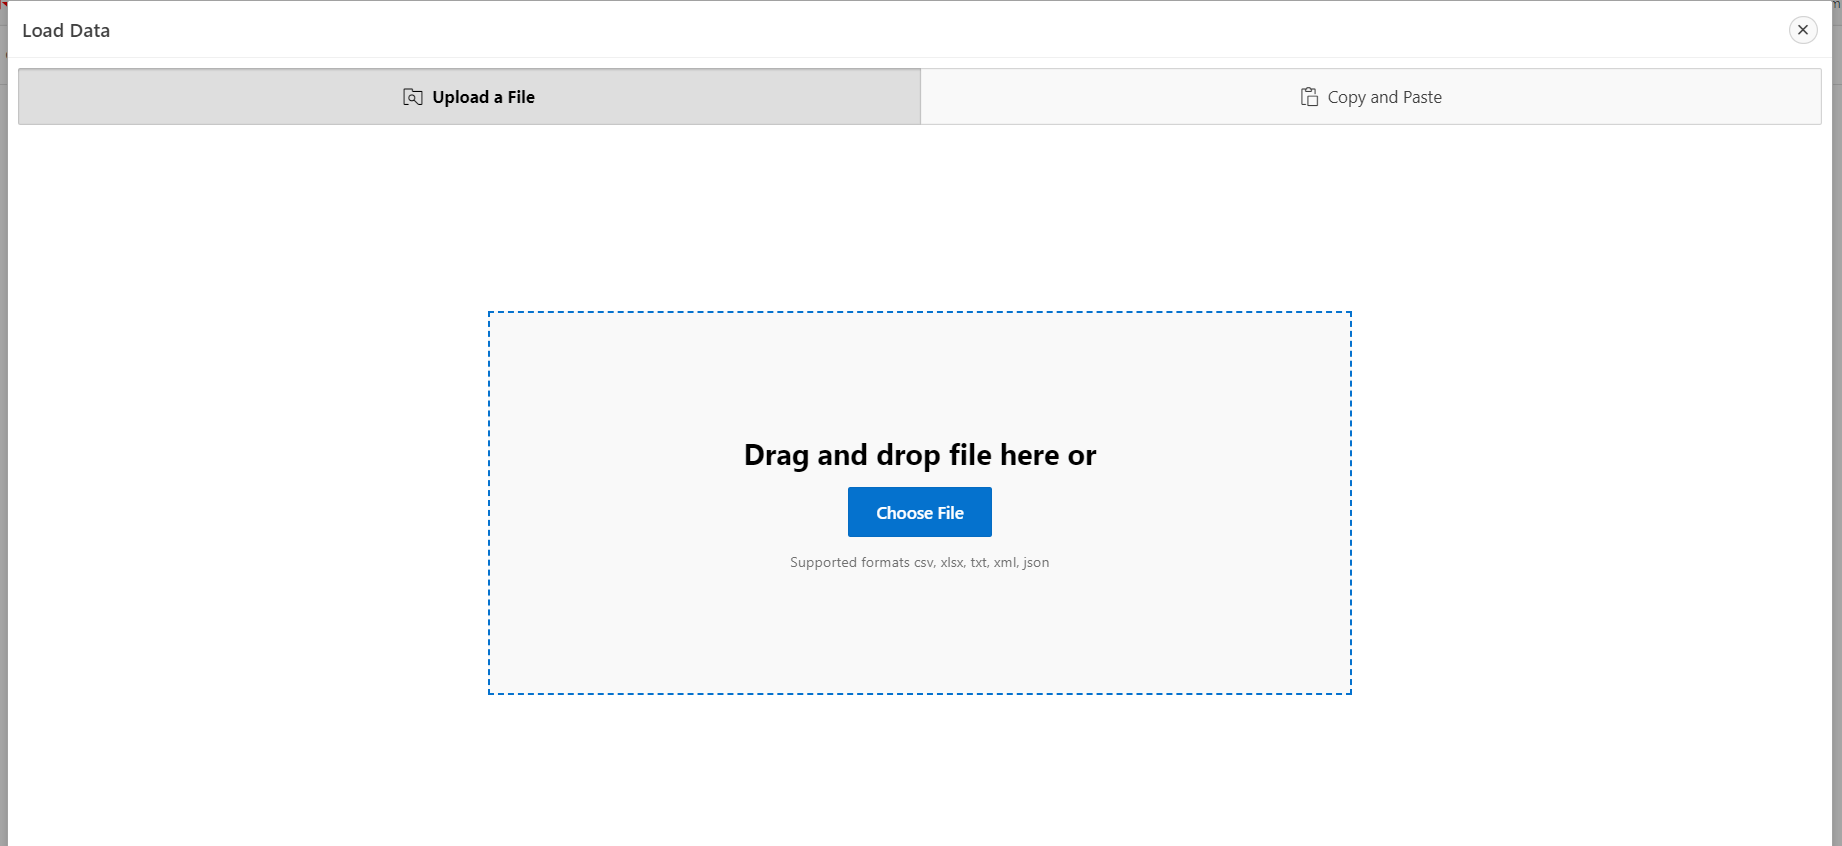
\includegraphics [width=8cm]{figure/Capture14.PNG}
        \caption{Caption}
        \label{capture3}
    \end{figure}
    
    \item Isi "table name" yang akan kalian buat, setelah terisi maka "table name error" akan otomatis terisi, lalu klik "load data"
     \begin{figure}[!htbp]
        \centering
        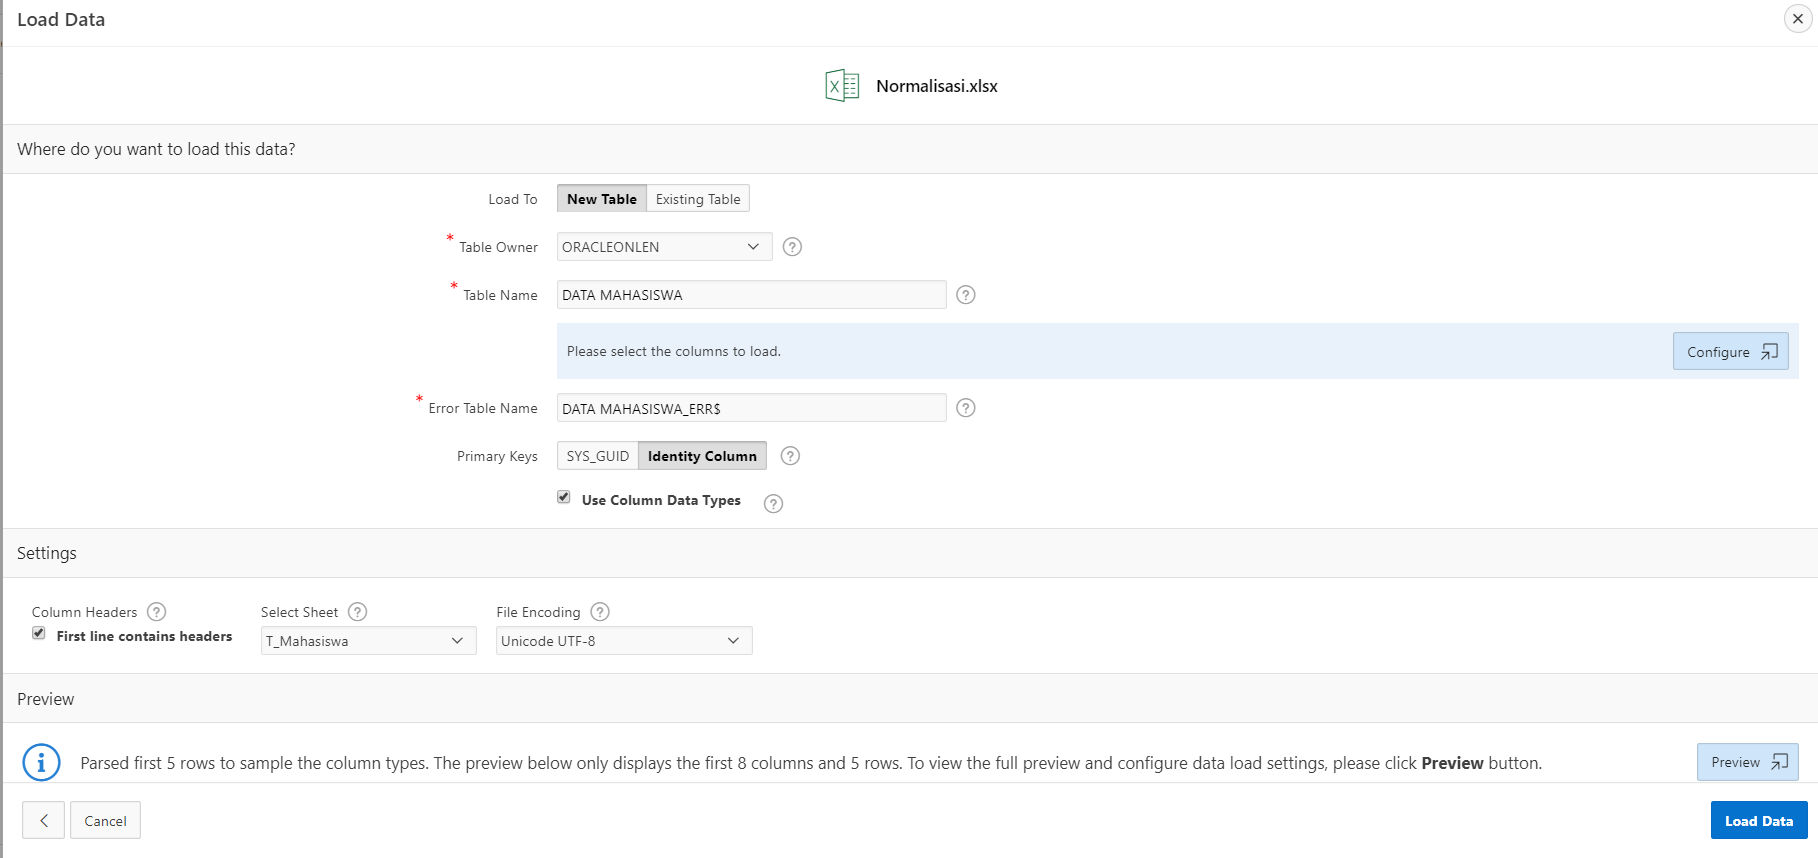
\includegraphics [width=9cm]{figure/Capture15.PNG}
        \caption{Caption}
        \label{fig:my_label}
    \end{figure}
    
    \item Setelah klik "Load Data", maka jika berhasil akan ada ceklis 
     \begin{figure}[!htbp]
        \centering
        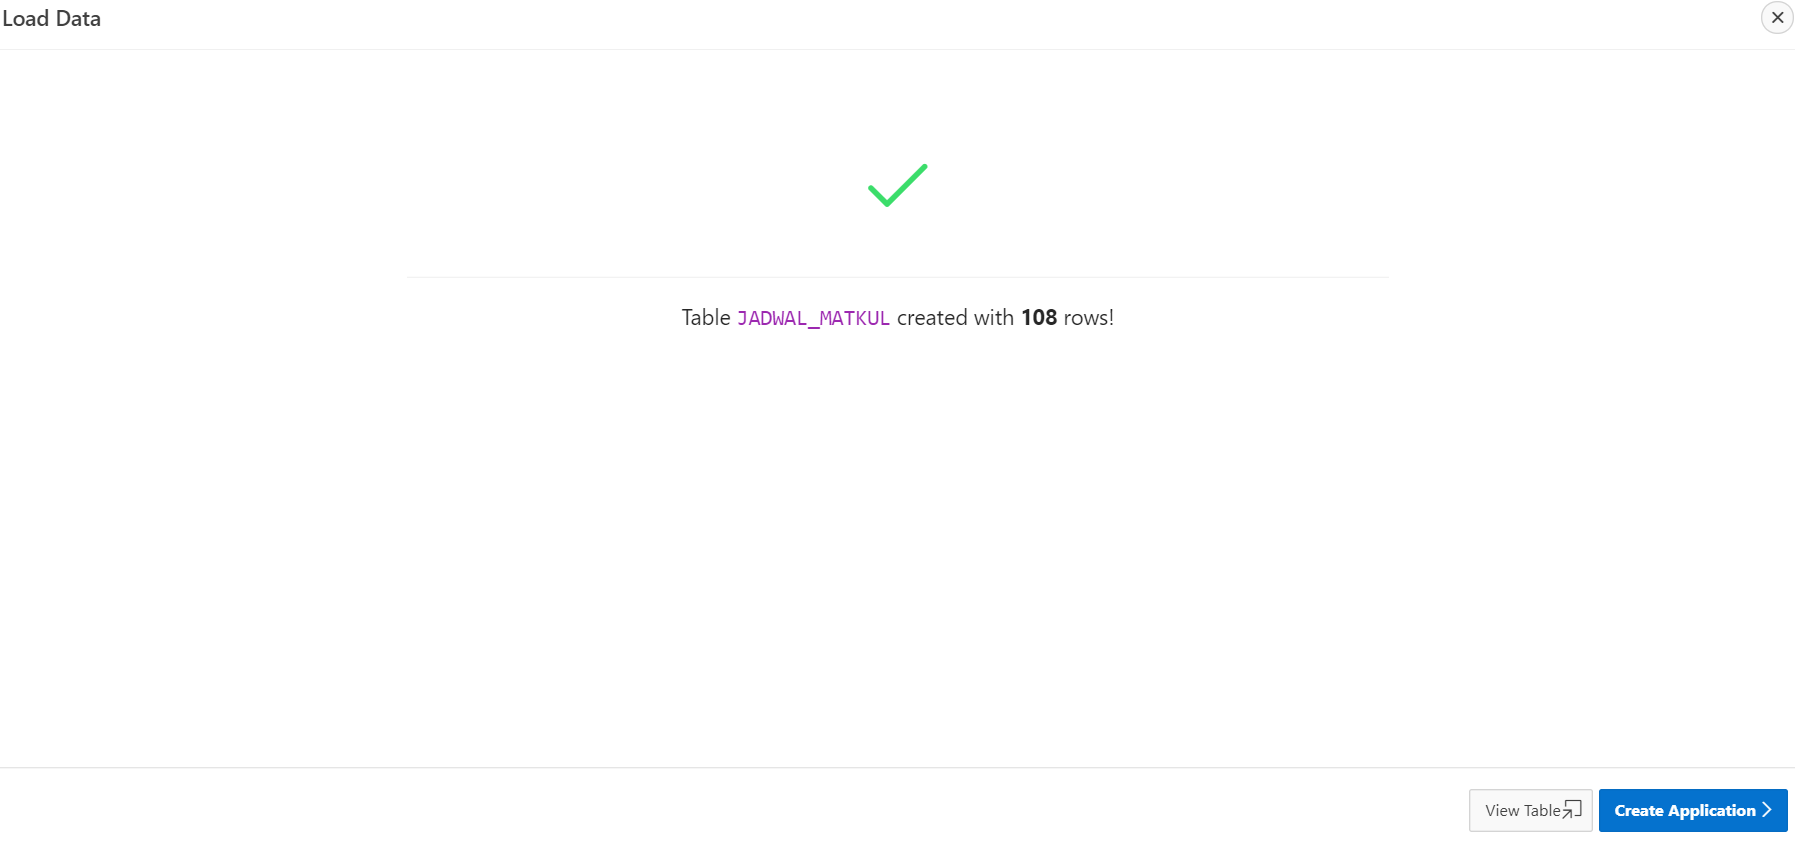
\includegraphics [width=9cm]{figure/Capture5.PNG}
        \caption{Caption}
        \label{fig:my_label}
    \end{figure}
    
    \item Setelah itu, buka tabel yang kalian buat, lalu drop column ID karena primary key dari tabel yang saya buat buka ID
     \begin{figure}[!htbp]
        \centering
        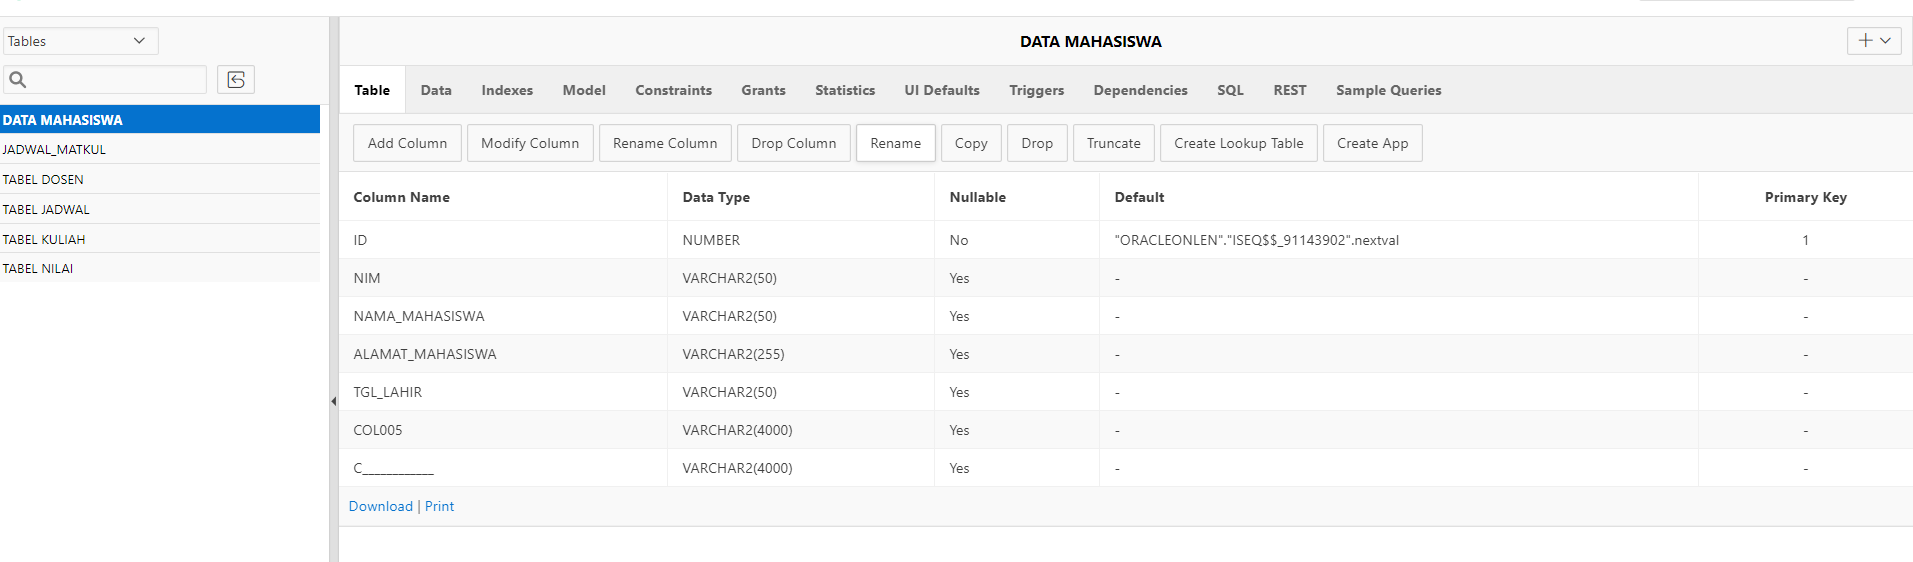
\includegraphics [width=14cm]{figure/Capture16.PNG}
        \caption{Caption}
        \label{fig:my_label}
    \end{figure}
    
    \item Pilih column ID buat di drop column
     \begin{figure}[!htbp]
        \centering
        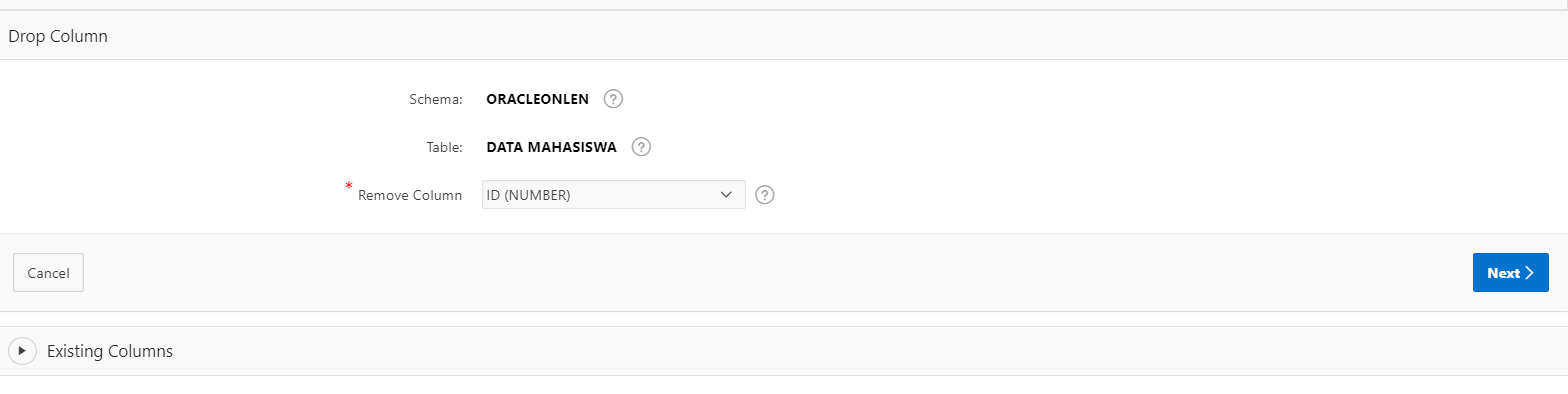
\includegraphics [width=14cm]{figure/Capture17.PNG}
        \caption{Caption}
        \label{fig:my_label}
    \end{figure}
    
    \item Buat Primary key pada tabel mahasiswa, dosen, dan kuliah
    \begin{figure}[!htbp]
        \centering
        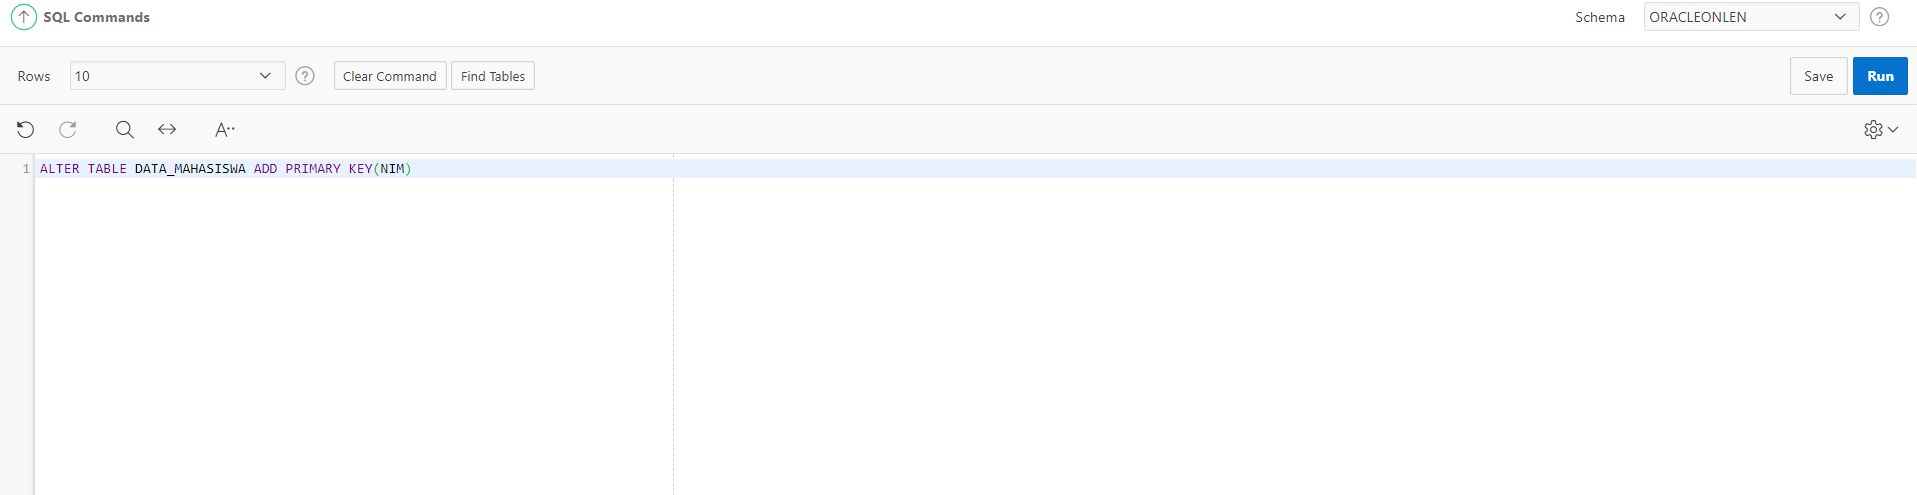
\includegraphics [width=9cm]{figure/Capture19.PNG}
        \caption{Caption}
        \label{fig:my_label}
    \end{figure}
    
    \item Buat Foreign Key 
    \begin{figure}[!htbp]
        \centering
        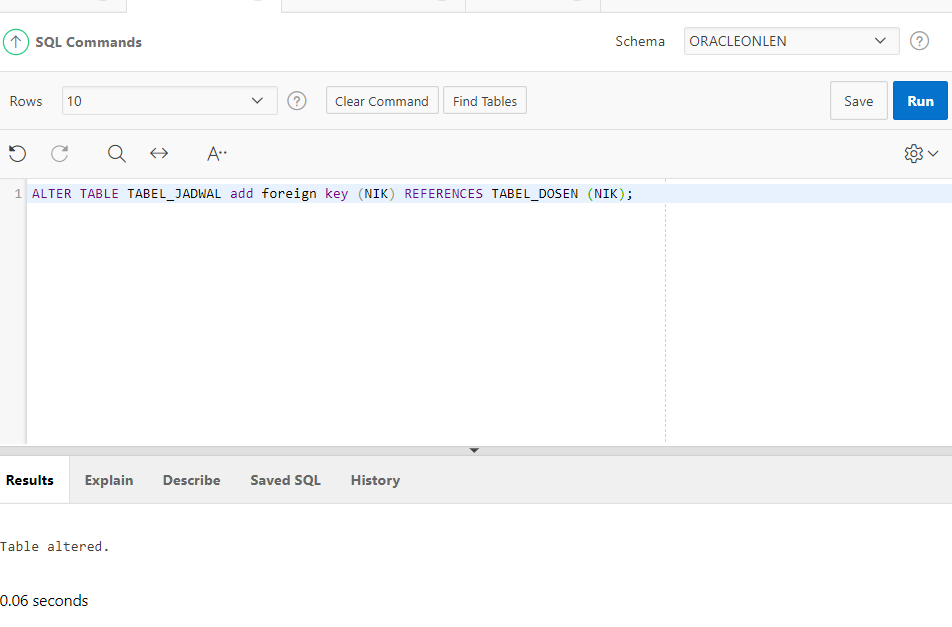
\includegraphics [width=9cm]{figure/Capture20.PNG}
        \caption{Caption}
        \label{fig:my_label}
    \end{figure}
    
    \item Setelah dibuatkan primary dan foreign key maka buka app builder dan pilih create lalu Creat Application
    \begin{figure}[!htbp]
        \centering
        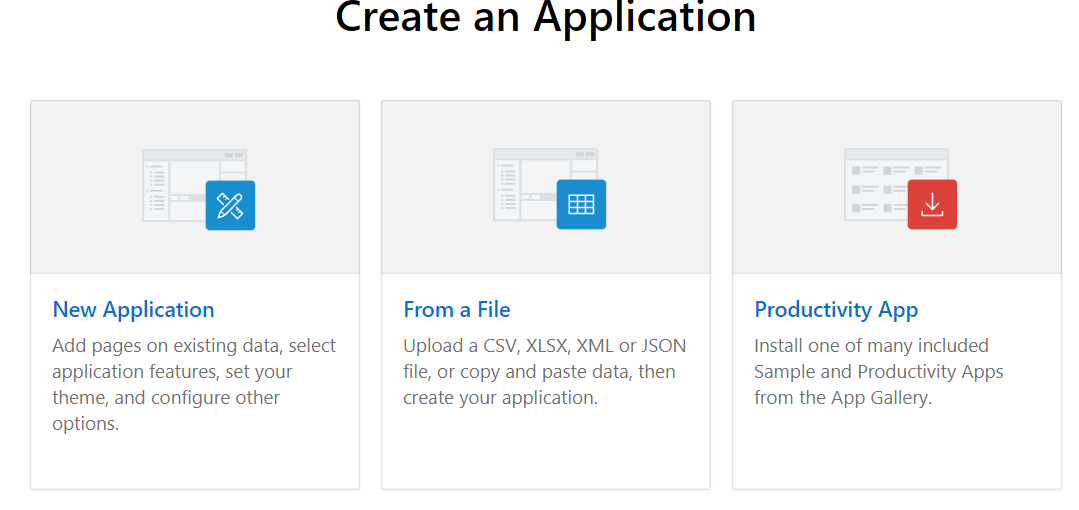
\includegraphics [width=9cm]{figure/Capture2.PNG}
        \caption{Caption}
        \label{fig:my_label}
    \end{figure}
    
    \item Pilih Add Page dan klik Interactive Report
     \begin{figure}[!htbp]
        \centering
        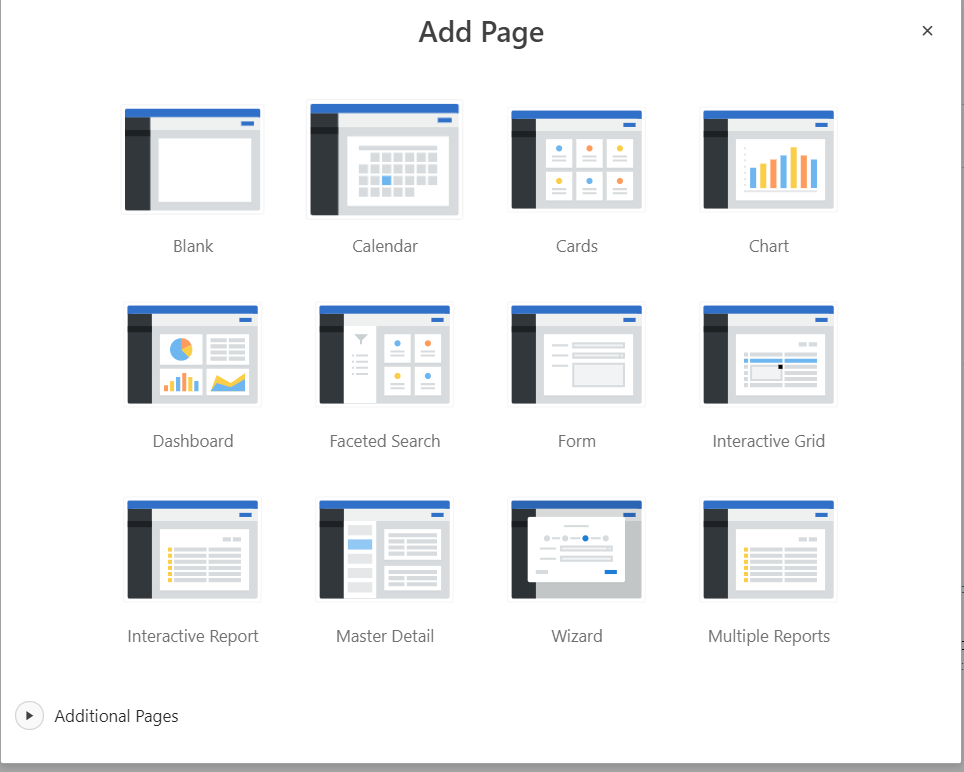
\includegraphics [width=5cm]{figure/Capture21.PNG}
        \caption{Caption}
        \label{fig:my_label}
    \end{figure}
    
    \item Masukkan Tabel yang telah dibuat 
     \begin{figure}[!htbp]
        \centering
        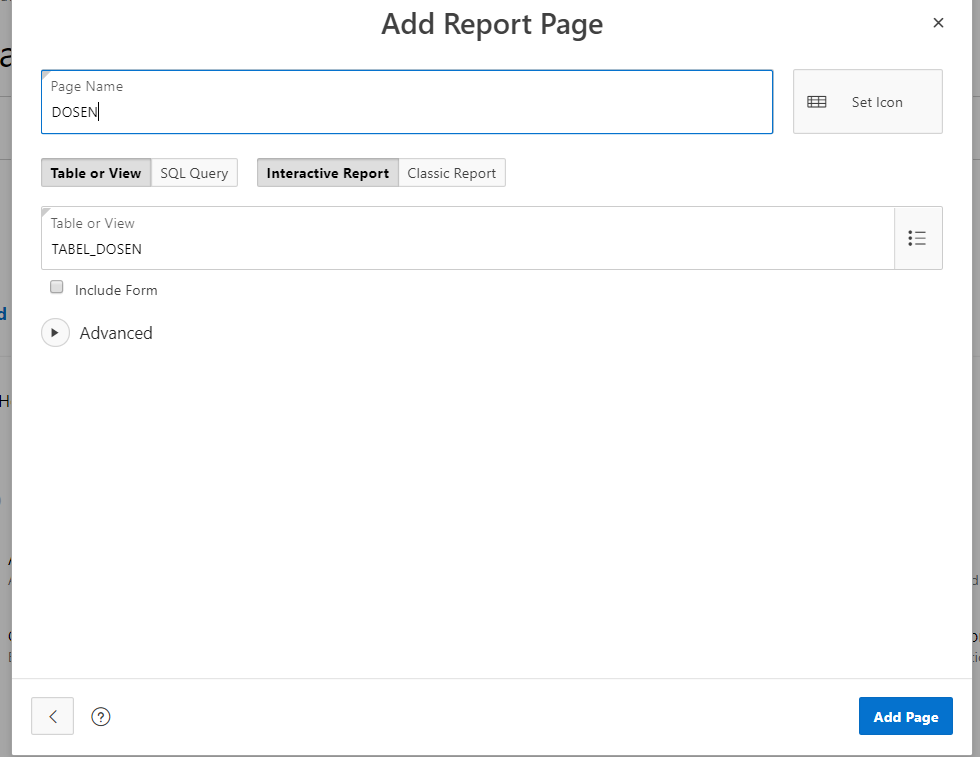
\includegraphics [width=5cm]{figure/Capture22.PNG}
        \caption{Caption}
        \label{fig:my_label}
    \end{figure}
    
    \item Setelah semua tabel dimasukkan, namai aplikasi sesuai hati kalian
     \begin{figure}[!htbp]
        \centering
        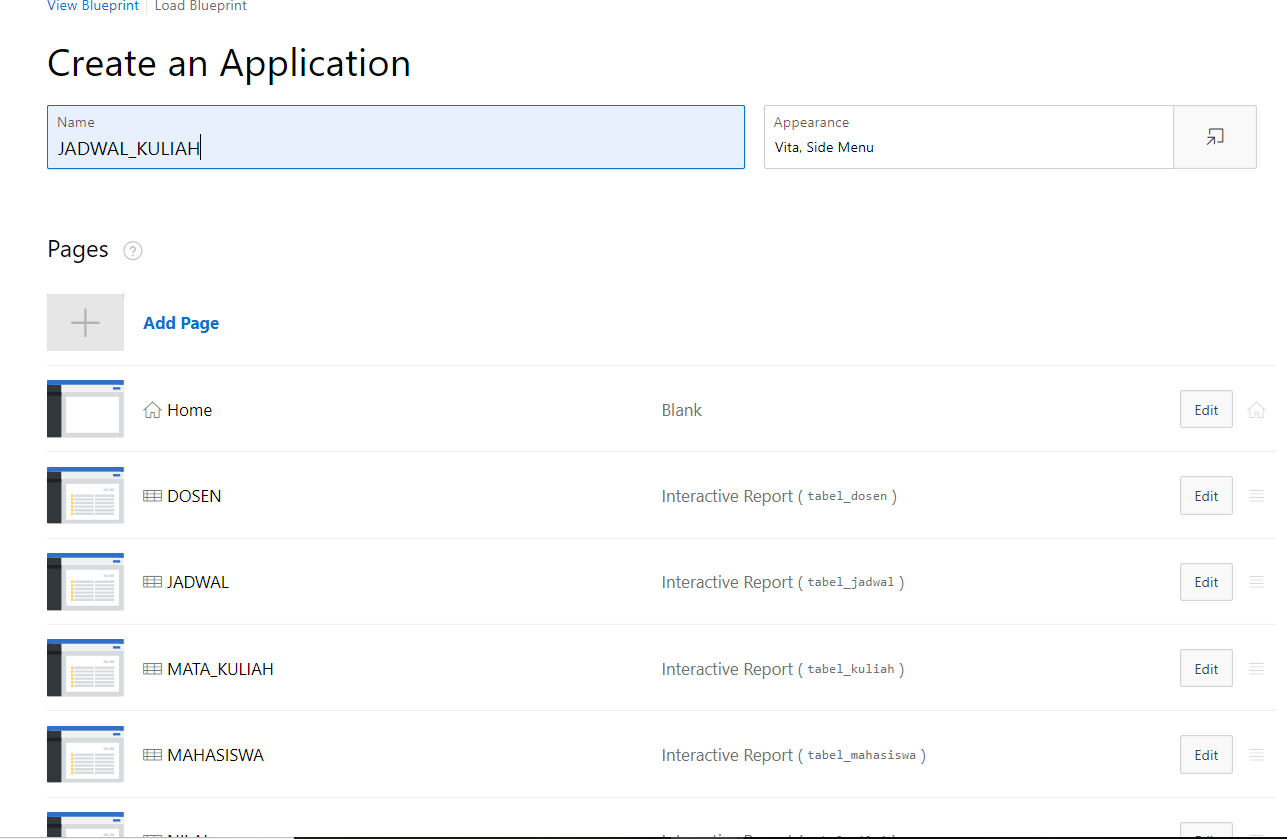
\includegraphics [width=7cm]{figure/Capture23.PNG}
        \caption{Caption}
        \label{fig:my_label}
    \end{figure}
    
    \item Sebelum masuk ke aplikasi yang telah dibuat, kalian harus login dulu terlebih dahulu memakai akun masuk oracle APEX
     \begin{figure}[!htbp]
        \centering
        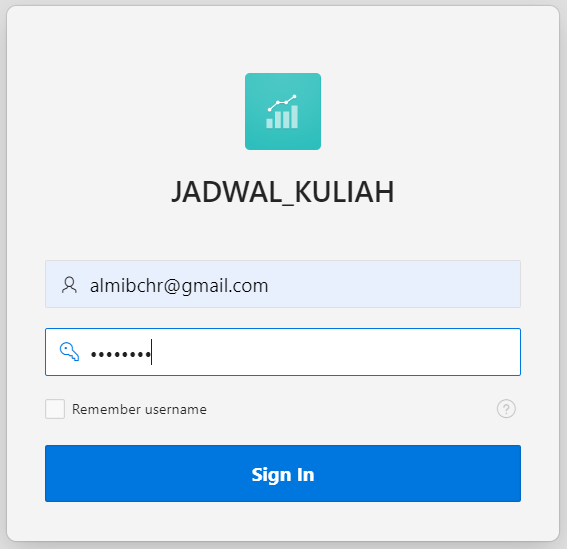
\includegraphics [width=7cm]{figure/Capture24.PNG}
        \caption{Caption}
        \label{fig:my_label}
    \end{figure}
    
    \item Setelah login maka akan masuk ke tampilan awal aplikasi yang telah dibuat
     \begin{figure}[!htbp]
        \centering
        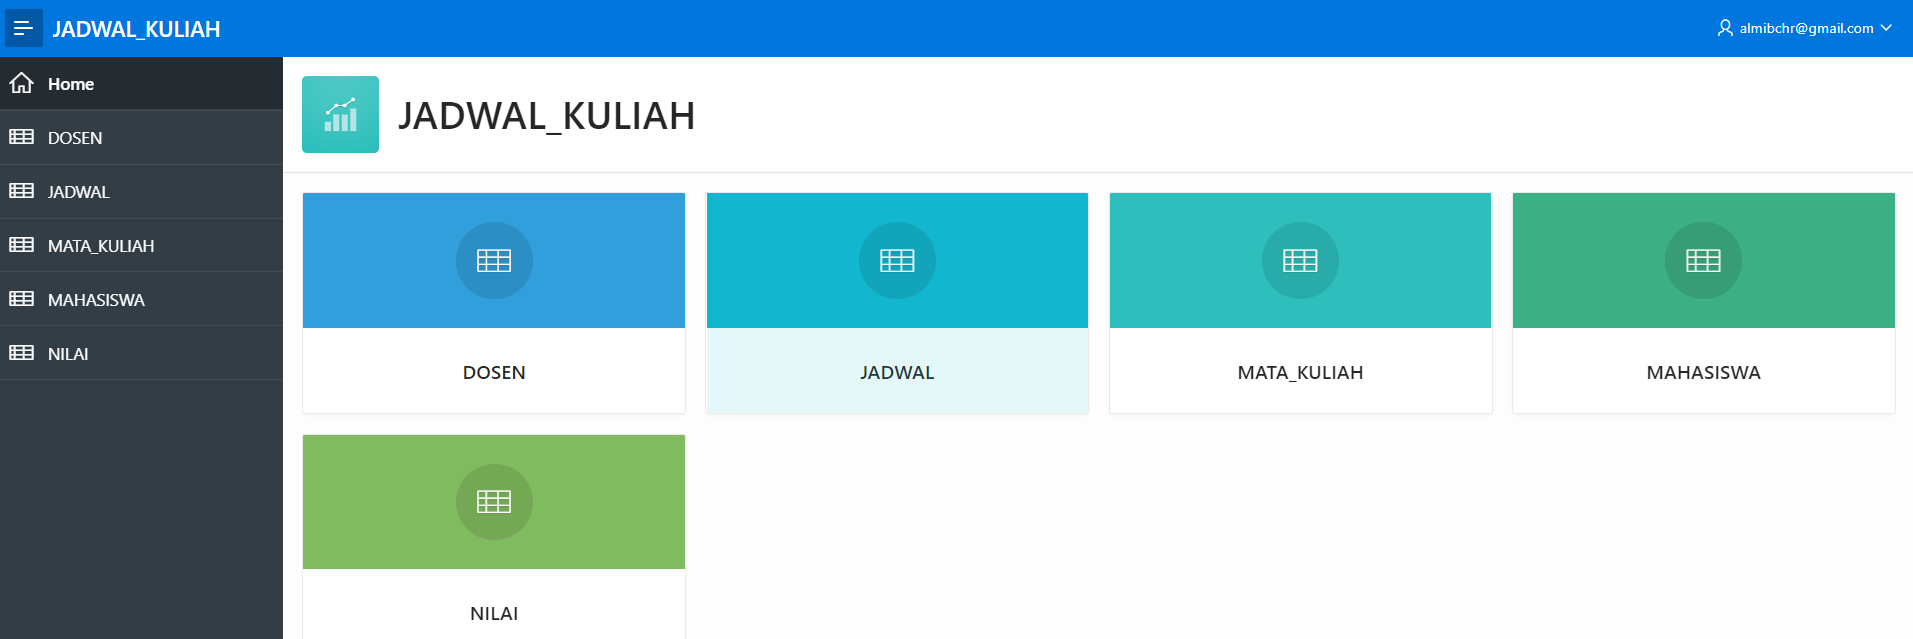
\includegraphics [width=7cm]{figure/Capture25.PNG}
        \caption{Caption}
        \label{fig:my_label}
    \end{figure}
    SELESAI !
\end{enumerate}
Link :  https://apex.oracle.com/pls/apex/f?p=93353:LOGIN\textunderscore DESKTOP:708449722230200:::::
Username : almibchr@gmail.com
\par
Password : almi2405
\end{document}

